\documentclass[Main.tex]{subfiles}

\begin{document}
\section{Spatial Models}\label{sec:spatial}
So far we have discussed characterization robot controllers and their corresponding PFSMs using rate equations. As Hamann and W\"{o}rn\cite{Hamann2008} point out, ``A drawback of these rate equations is the limited representation of space---either homogeneous space is assumed or a coarse discretization by states is done.'' Indeed, during our discussion of macro-model development we assumed a uniform starting distribution of robots and interaction objects (such as sticks) in an arena. We also defined random walk as being the process by which this uniform distribution of agents was maintained during the course of the experiment and completely ignored physical properties such as the maximum distance a robot could move per time step due to it's velocity. The process of random walk effectively allowed us to \emph{teleport} robots within the arena at any time, thereby simplifying our mathematical model to a system of ODEs. While these assumptions are justified because our aim in designing the macro-model is to study the overarching properties of the swarm system without worrying about the dynamics of individual agents, such non-spatial descriptions of the swarm system are bound to introduce unintended side-effects (such as \emph{teleportation}) in our results. Non-spatial models also make modeling of agent interactions such as collisions and ranged communication more complicated. To account for these inaccuracies in non-spatial models, the concept of spatial modeling of swarm robot systems has evolved into a research topic in the last decade.

Spatial models for studying robot swarms have been adopted from older, well-studied models in physics. Specifically, spatial models of swarm systems are heavily influenced from models of Brownian motion of particles and share a lot of the same mathematics and theory. A brief history of the mathematical solution of Brownian motion follows as it sheds light on the evolution of spatial models over time. 

Robert Brown first discovered the phenomenon of Brownian motion in 1828 when he observed seemingly random movements of particles within vacuoles of pollen grains. The term ``Brownian Motion'' was coined later, in his honor, and is used to describe the motion of larger particles due to their constant collisions with smaller molecules of the medium within which they are suspended, e.g. The random movement of dust particles in still air, crushed tea leaves in a glass of water, etc. It wasn't until the turn of the next century when, in 1905, Einstein mathematically solved the phenomenon of Brownian motion. Independent solutions were subsequently discovered by Smoluchowski (1906) and Langevin (1908). The Langevin equation is used as the basis for swarm system micro-models as it is a simpler and more adaptable approach than the other two. Then in 1914 and 1917, Fokker and Planck respectively analyzed the probability distribution of the velocity of diffusing particles by deriving a PDE, now well known as the Fokker-Planck equation. This equation is used as the basis for a macro-model in swarm system analysis. The Fokker-Planck equation is also sometimes known as the Kolmogorov forward equation as it is a special case of a more general equation used to describe time and state continuous Markov processes, invented by Kolmogorov in 1931. Finally, in 2003 Schweitzer introduced the concept of free agents or active particles experiencing Brownian motion, capable of producing energy internally and using it for self propulsion; much like swarm robots. For these reactive agents, generalized Langevin and Fokker-Planck equations have been subsequently developed and we will discuss them next.

\subsection{Langevin Equation: A Microscopic Model}
Like non-spatial models, spatial models for robot swarms can be split up into two system resolutions --- the micro-level and the macro-level. We will begin our discussion of spatial modeling at the micro-level using a Langevin equation because the macro-level Fokker-Planck equation can be derived from it. It is important to note that a Langevin equation is any differential equation that describes the temporal and spatial evolution of a subset of the degrees of freedom of a particle, i.e. it is not a single equation but a class of equations that all describe the same phenomenon. The original equation for a Brownian agent by Langevin was of a different form than the one we will be using to study robot swarms as it did not take into consideration the case where an agent could move due to some internal driving force, as robots do. A derivation from Langevin's original equation to the modified form seen below is available in Hamann's dissertation work\cite{Hamann2010}.
\begin{equation}\label{eq:lan}
\V{R}'(t) = -\V{A}(\V{R}(t),t) + B(\V{R}(t),t)\V{F}(t)
\end{equation}
In Eqn.~\eqref{eq:lan}, $\V{R}(t)$ represents the position of the agent at time-$t$, $\V{A}(\V{R}(t),t)$ is a direction function describing the agent's deterministic motion, while $B(\V{R}(t),t)\V{F}(t)$ describes the agent's random motion based on $\V{F}$, a stochastic process (white noise). $\V{A}$ is commonly referred to as the \emph{drift} term in the equation and $B$, the \emph{diffusion coefficient}. $\V{F}(t)$ is a normalized noise term ($\norm{\V{F}(t) = 1}$) with 0 mean and is uncorrelated in time ($\left<\V{F}(t)\V{F}(t') = \delta(t - t')\right>$). Using constant values for drift and diffusion in 1 spatial dimension, Figure~\ref{fig:lan} shows the movement of a robot (or particle) solved using Eqn.~\eqref{eq:lan}.

\begin{figure}[!ht]
\centering\begin{subfigure}{.5\textwidth}
\centering\includegraphics[width=7cm]{assets/LanNoDrift.png}
\end{subfigure}~
\centering\begin{subfigure}{.5\textwidth}
\centering\includegraphics[width=7cm]{assets/LanDrift.png}
\end{subfigure}
\caption{Left: Solution to Langevin equation for a particle in 1D with $\V{A} = 0$, i.e. no drift. Right: Solution with $\V{A} = 0.1$. In both cases the diffusion coefficient is constant, $B = 0.3$, and $\V{F}$ uses an uncorrelated normal distribution with mean $\left<\V{F}\right> = 0$.}\label{fig:lan}
\end{figure}

\subsection{Fokker-Planck Equation: A Macroscopic Model}
From the Langevin equation used in the previous section, we can derive the Fokker-Planck equation as stated below,
\begin{equation}
\PD{\rho(\V{r},t)} = -\nabla(\V{A}(\V{r},t)\rho(\V{r},t))+\frac{1}{2}Q\nabla^2(B^2(\V{r},t)\rho(\V{r},t))
\end{equation}
\begin{figure}[!ht]
\centering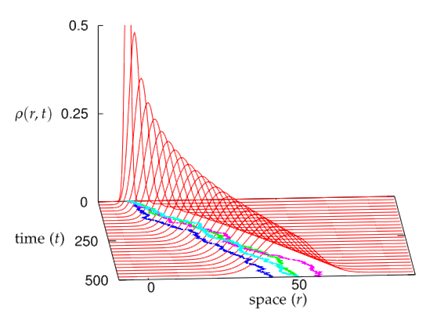
\includegraphics[width=7cm]{assets/fokkerPlanck.png}
\centering\caption{A visual comparison between the spatial micro vs. macro-level equations. The colored lines on the $r$-$t$ plane show the paths taken by individual particles, found via the Langevin equation, while the overarching red curve is the probability distribution for the entire ensemble as described by the Fokker-Planck equation.}\label{fig:fokkerplanck}
\end{figure}

A clear and concise derivation of the above equation from the Langevin equation is provided in section 4.1 of \cite{Hamann2010}, which in turn follows closely from the book \emph{Synergetics} by Haken (1977). The terms $\V{A}$, $B$ and $\V{F}$ reprise their earlier roles from the Langevin equation, while $Q$ is a new displacement term due to collisions between particles. $\rho(\V{r}, t)$ is the probability of encountering a particle at position $\V{r}$ and time $t$. As one can see, the Fokker-Planck equation gives us a \emph{probability distribution} of the positions of particles in space, making it a viable macroscopic model compared to the micro-level Langevin equation which gives us the \emph{position} of a \emph{single} particle in space (see Figure~\ref{fig:fokkerplanck}).

\subsection{Applications}
The Fokker Planck equation is a relatively new tool in the field of swarm robot modeling and has notably been used by Hamann\cite{Hamann2008,Hamann2010}, as well as Prorok, Correll and Martinoli\cite{Prorok2011} in their work on boundary coverage and inspection of jet-turbine engines using swarms of miniature robots. They used a hybrid approach for modeling collective inspection that involves a probabilistic non-spatial model coupled with spatial micro-macro diffusion equations for modeling collective inspection of regular structures to improve consensus with observed experimental values. 

\begin{figure}[!ht]
\centering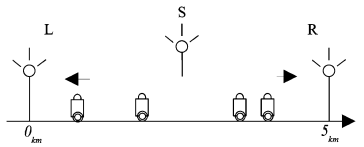
\includegraphics[width=8.5cm]{assets/spatSignal.png}
\centering\caption{Experiment setup for centralized robot population control experiment proposed by Milutinovi\`{c} and Lima in%\cite{Milutinovi2006}
.}\label{fig:signal}
\end{figure}

A spatial model is used in\cite{Milutinovi2006} to control a large scale multi-agent system using centralized controller and three signal sources. The goal of this experiment is to show successful control of a large population of robots by collectively moving them along a 1-dimensional arena using \emph{left}, \emph{right} and \emph{stop} signals from a moving aerial controller. The model accounts for the fact that not all robots receive the signal or change direction/move promptly upon successfully receiving a signal. A visual representation of this setup can be seen in Figure~\ref{fig:signal}.

Although the Fokker-Planck equation is not mentioned explicitly in\cite{Milutinovi2006}, the authors employ the use of a system of PDEs to predict the position of the swarm in the arena via a probability density function (PDF). Their approach is therefore rather similar to the macro-level spatial modeling approach described earlier in this paper. The goal of moving the entire swarm  from point A to point B in a 1D arena just through the use three signals controlled by a centralized controller is formulated as an optimal control problem by the authors. It is solved by introducing appropriate weighting and cost functions to the PDEs and computing the PDF at any given time to predict the collective motion/position of the swarm. The control signals are then switched accordingly to move the swarm in a desired direction. Two particularly insightful plots (Figures 4 \& 5) are provided in\cite{Milutinovi2006} that showcase this result, i.e. the PDF evolution of stopped and moving robot populations as time progresses.

While the non-spatial modeling approaches we have discussed so far use a phenomenological approach to construct the macro-model equations, this is not a viable option in the spatial model case. Typically, the drift and diffusion coefficient functions in the Fokker-Planck equation are adapted based on the swarming task we attempt to model but constructing these functions is not as straightforward as defining the rate equations from a robot controller, as seen in the non-spatial case. The $\V{A}$ and $B$ functions of the Fokker-Planck equation serve to bridge the gap between micro-level and macro-level observations of a swarm system and hence provide quite a challenge to design accurately.
\end{document}